

\begin{center}
\begin{figure*}
\begin{tabular}{c}
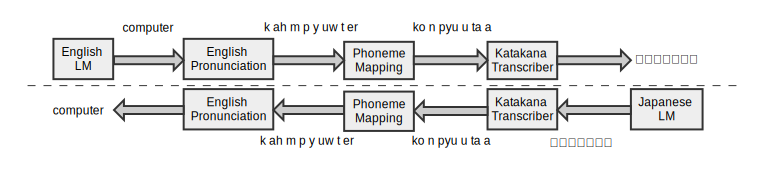
\includegraphics[scale=0.6]{figures/fsts}\tabularnewline
\end{tabular}\caption{\label{font-table} Transliteration generative story as an FST cascade. Top: transliteration of the word ``computer'' to Japanese. Bottom: the reverse process. Each box represents a transducer. During training, only the phoneme mapping models are estimated while keeping the other models fixed.}
\label{fig:fsts}
\end{figure*}
\end{center}


In the following two sections we show that PAT leads to better transliteration models even without parallel data. We first briefly describe a generative model for transliterated terms, due to Knight and Graehl, and subsequently report the results of a carefully designed decipherment experiment.

\subsubsection{Deciphering Transliterations}

Transliteration is a mapping of terms between writing systems of different languages. 
Usually, the transliterator tries to preserve the sound of a term as it is spoken in the original language. For example, the word ``computer'' in Japanese is transliterated to Japanese as ``ko n pyu u ta a'' (in Romaji). 
The \emph{back-transliteration} task asks to reverse this process by restoring transliterated foreign words to their original script.

Knight and Graehl \cite{KG98} model the transliteration of an English
term $w$ into a Japanese $k$ using a generative story, encoded as
a cascade of four finite state transducers (see Figure \ref{fig:fsts}): 
\begin{enumerate}
\item First, a word $w$ is generated according to an English language model
$P_0[w]$
\item $w$ is then mapped to a sequence of English
phonemes $(e_{1},\ldots,e_{M})$ according to a pronunciation model
\item Each phoneme $e_{m}$ is mapped to a sequence of Japanese phonemes
$j_{m}$ according to a phoneme mapping model $P_0[j_{m}\mid e_{m}]$
(in practice, restricted to 1-to-1 or 1-to-2 phoneme mappings)
\item Finally, the entire Japanese pronunciation sequence is mapped to a
Japanese word $k$ in Katakana script
\end{enumerate}
Knight and Graehl (\cite{KG98}) construct and train these FSTs independently. 
In particular, to train the phoneme mapping model $P_0[j_{m}\mid e_{m}]$ a parallel
phoneme corpus $\{(w_{n},\, k_{n})\}$ is prepared and its likelihood is then maximized using EM.

However, collecting parallel data is often a time consuming and laborious process.
To combat the need for parallel data Ravi and Knight \cite{RK09} suggest learning to transliterate in the \emph{deciphermenet} setting:
In decipherment, only Japanese words $K=\{k_{n}\}_{n=1..|K|}$ need be collected. 
Treating its English origin as missing data, a Japanese word $k$ is then viewed as being generated by all English words $w$ in the language model via the marginalization equation $P[k]=\sum_{w}P_0[w]\cdot P_0[k\mid w]$.
In this case, the data log-likelihood takes the form:
\begin{align*}
log P_0[K]& = \sum_n log \sum_{w} P_0[w] \cdot P_0[k_n\mid w]
\end{align*}

%We note a few points:
%\begin{itemize}
%\item The computational cost of solving this problem is much higher than the parallel case since we are forced to use the language and pronunciation models during training time. 
%\item Only the phoneme mapping parameters $P[j_{m}\mid e_{m}]$ are trained while
%the other FSTs' parameters are kept fixed.
%\end{itemize}

\subsubsection{Parameter Agreement Training}
The generative story above describes how English is transliterated to Japanese.
To apply PAT, we first require a model that generates English from transliterated Japanese.
To do so, we simply reverse the generative story - we first sample the word $k$ from a Japanese language model (estimated over Katakana only) and proceed using the inverse FSTs, in the reverse order.
Training the resulting model in the decipherment setting amounts to collecting a (monolingual) English corpus $W=\{w_n\}_{n=1..|W|}$ and then maximizing its log-likelihood $log P_1[W]$.

Finally in PAT, we maximize the regularized objective function:
\begin{align*}
log P_0[K] + logP_1[W] + \lambda R(P_0, P_1)
\end{align*}


%Overall, less than 200 parameters have value larger than 0.01 in the parallel case, while
%in decipherment, the number orders on 400. As expected, ordinary EM
%leaves a lot of room for ambiguity in the decipherment case.


\begin{center}
\begin{figure*}[t]
\begin{tabular}{ccc}
 &  & \tabularnewline
 & 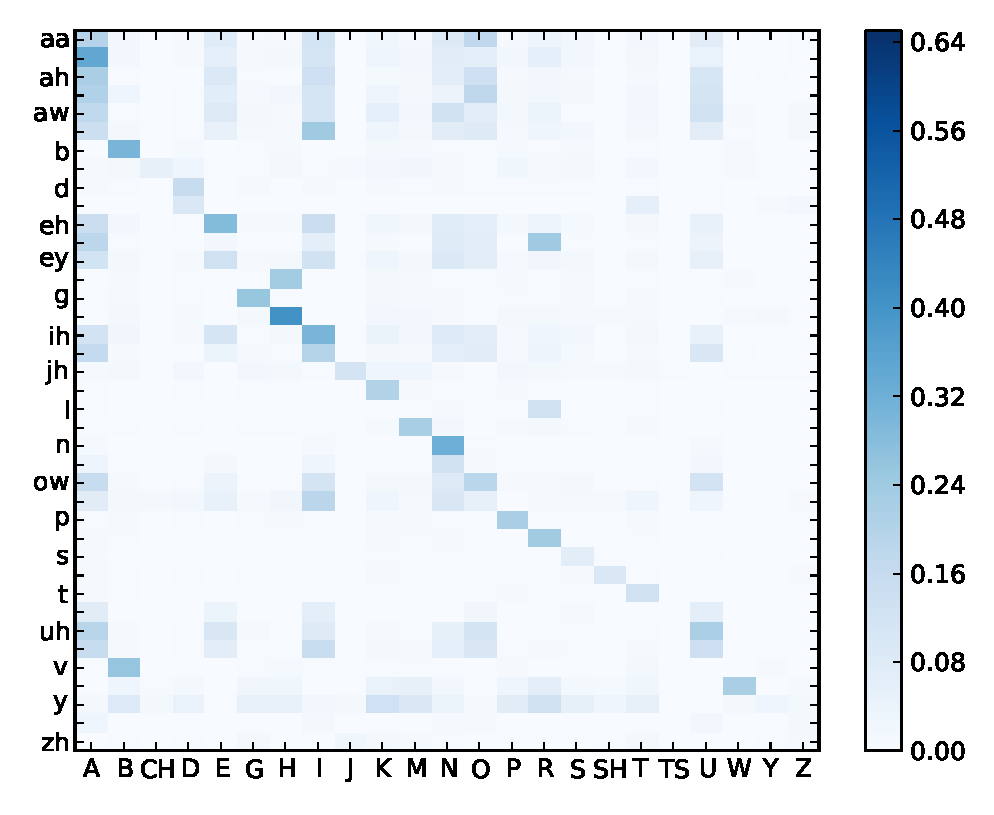
\includegraphics[scale=0.4]{figures/model_11_vanilla} & \includegraphics[scale=0.4]{figures/model_11_gm}\tabularnewline
 &  & \tabularnewline
\end{tabular}
\caption{\label{font-table} The 1-to-1 phoneme mapping submatrix of the model learned by ordinary EM (left) and parameter agreement with the geometric mean regularizer. Parameter agreement produces sparser models.}
\end{figure*}
\end{center}

\subsubsection{Deciphering Transliterations - Experiments}

Ravi and Knight (\cite{RK09}) compare back-transliteration whole-name error rates (WNER) on
a list of 100 US senator names (In WNER, a decoding is correct if both the first and last name are decoded correctly).
They report 40\% error rate in the
parallel setting, and a 73\% error rate when using their best decipherment setting.

In order to compare PAT against independent training, we produced similar decipherment setting as in \cite{RK09}. Specifically, used the following Language Models (LM) and FSTs:
\begin{itemize}
\item Two unigram language models over terms: a ~40K English LM estimated over the most frequent capitalized words from the gigaword corpus, and a ~25K Japanese LM, estimated over the most frequent Katakana terms in the Japanese news 2005-2008 Leipzig Corpora (http://corpora.informatik.uni-leipzig.de/download.html)
\item English and Japanese pronunciation FSTs. The English pronuncation model was constructed using the CMU pronunciation dictionary. A Japanese pronunciation models was hand built.
\end{itemize}
Note that these LM and FSTs require only monolingual knowledge to create.


\begin{itemize}
\item no Parallel Data
\item Fair Experiment setting

\begin{itemize}
\item Data Collection, Numbers
\item Generate the entire LM both ways.
\item Comparison of results and sparsity, image for sparsity
\end{itemize}
\end{itemize}